\documentclass[pra,showkeys,twocolumn,showpacs]{revtex4-1}
\usepackage{amsmath}
\usepackage{amsfonts}
\usepackage{amssymb}
\usepackage{array}
\usepackage{color}
\usepackage{soul}
%\usepackage{floatflt}
\usepackage{graphicx}
\DeclareMathOperator{\tr}{Tr}
\newcommand*{\eq}[1]{(\ref{#1})}
\newcommand*{\eqs}[2]{(\ref{#1})--(\ref{#2})}
\newcommand{\exi}{\tr{\{e^{-\frac\beta2\sum_k\lambda_k\gamma_k^\dag\gamma_k}\}}}
\renewcommand{\l}{\left(}
\renewcommand{\r}{\right)}

\begin{document}
\title{Quantum-assisted unsupervised data clustering}

\author{I.~D.~Lazarev} 
\affiliation{Institute of Problems of Chemical Physics of Russian Academy of Sciences, Acad. Semenov av. 1, Chernogolovka, Moscow Region, Russia, 142432}
\affiliation{ Faculty of Fundamental Physical-Chemical Engineering, Lomonosov Moscow State University, GSP-1, Moscow, Russia 119991}

\author{Marek Narozniak}
\affiliation{New York University Shanghai, 1555 Century Ave, Pudong, Shanghai 200122, China}
\affiliation{Department of Physics, New York University, New York, NY, 10003, USA.}

\author{Tim Byrnes}
\affiliation{New York University Shanghai, 1555 Century Ave, Pudong, Shanghai 200122, China}
\affiliation{State Key Laboratory of Precision Spectroscopy, School of Physical and Material Sciences, East China Normal University, Shanghai 200062, China}
\affiliation{NYU-ECNU Institute of Physics at NYU Shanghai, 3663 Zhongshan Road North, Shanghai 200062, China}
\affiliation{National Institute of Informatics, 2-1-2 Hitotsubashi, Chiyoda-ku, Tokyo 101-8430, Japan}
\affiliation{Department of Physics, New York University, New York, NY 10003, USA}


\author{A.~N.~Pyrkov} 
\email{Email address:pyrkov@icp.ac.ru}
\affiliation{Institute of Problems of Chemical Physics of Russian Academy of Sciences, Acad. Semenov av. 1, Chernogolovka, Moscow Region, Russia, 142432}


\date{\today}

\begin{abstract}
Unsupervised machine learning is one of the main techniques in artificial intelligence. Quantum computers offer opportunities to speed up such machine learning techniques, where the number of input data elements is extremely large. Here, we propose a realization of quantum assisted unsupervised data clustering using the self-organizing feature map artificial neural networks. We make a proof-of-concept realization of one of the central components of the approach on the IBM Q Experience and show that it allows us to reduce number of calculations in a number of clusters. [TB: Explain what the main technique that is used is.  This is basically a QAOA hybrid quantum-classical approach right? If so, you should explain this] We compare the results with the classical algorithm on a toy example of unsupervised text clustering.  
\end{abstract}



%\pacs{}
\maketitle



\section{Introduction}
The combination of big data and artificial intelligence ---  dubbed the fourth industrial revolution --- has profoundly affected the modern economy in a plethora of different ways from robotics to agriculture \cite{Lecun2015, ghahramani2015,schwab2017,esteva2019, tyrsa2017}. Contemporary artificial intelligence methods based on neural networks also have the potential to enhance the role of novel analytical methods in science and engineering \cite{kaggle2014, radovic2018, butler2018, radovic2018}. Paradoxically, the exact mechanism of why neural networks are so powerful remain unknown (in many cases it is regarded as a black box).  It has been speculated that limits to the neural network approach based on the computational power of von Neumann architecture are being approached, and improvements appear only due to heuristic escalation of complexity \cite{marcus2018,sze2017,kourtis2020}.

In particular, the self-organizing feature map (SOFM) \cite{kohonen1990,kohonen1996,kohonen1997}, is a type of artificial neural network (ANN) that is trained in an unsupervised manner. SOFMs are used in many areas \cite{vilibic2016, guido1998, doszkocs1990, jones2012,mori2019,corsello2017,zhu2018,chea2016} and in comparison with many other artificial neural networks they apply competitive learning and preserve the topological properties of the input space \cite{kiviluotoa1996}. The SOFMs with a small number of nodes are similar to the K-means algorithm but for larger SOFMs they represent data in a fundamentally topological way that allows one to do dimensionality reduction.  Once it is trained, the map can classify a vector from the input space by finding the node with the smallest distance metric. 

Meanwhile, there has been much interest recently in applying quantum computing techniques to machine learning \cite{dunjko2018, biamonte2017, schuld2014, carleo2019}. The main focus of early works in quantum machine learning (QML) was on the use of quantum computers to perform basic linear algebra subroutines with a quantum speedup (such as Fourier transform and solving systems of linear equations \cite{wiebe2012,harrow2009,childs2017}) by utilizing quantum phenomena such as quantum entanglement and quantum superposition \cite{biamonte2017, schuld2014}.  Quantum versions were developed for linear regression, principal component analysis, support vector machine, K-means algorithm and others \cite{lloyd2013,lloyd2014,dunjko2016,paparo2014,rebentrost2014}. More recently, there has been attention on developing quantum neural networks \cite{kamruzzaman2019, schuld2014b, jeswal2019}. The interest in quantum neural networks was inspired by progress in experimental quantum computing when it became possible to use parametrized quantum circuits, where the parameters behave much like the weights of a neural network \cite{lewenstein1994}. In particular, quantum algorithms for training and evaluating feedforward neural networks was developed, which are one of the most usable neural network models \cite{allcock2018, tacchino2019}. Recent results connecting the classical Bayesian approach to deep learning allowed for the development of a new algorithm for Bayesian deep learning on quantum computers \cite{zhao2019}. The quantum models for convolutional neural networks, which may be suitable for the problems of learning of quantum states were also proposed \cite{cong2019, liu2019}. Quantum classification, tested on the MNIST dataset, via slow feature analysis based on the use of quantum Frobenius distance was proposed \cite{kerenidis2018}. Sublinear quantum algorithms for training linear and kernel-based classifiers were designed \cite{li2019}. Furthermore, continuous-variable quantum neural networks \cite{killoran2019}, quantum autoencoders \cite{bondarenko2019}, quantum approaches for reinforcement learning \cite{dunjko2017, nautrup2019, foesel2018} and some other \cite{rebentrost2018, purushothaman1997, verdon2019, cherny2019, byrnes2013, mishra2019, vinci2019, lu2019} were developed. Currently, it is believed that implementation of quantum neural networks can be the main test bed to achieve practical quantum supremacy on noisy intermediate scale quantum (NISQ) devices.

[TB: I think we definitely need to cite and describe hybrid quantum-classical approaches, like QAOA.  Could you please add several sentences and a solid set of references for these]

In this paper, we analyze  a hybrid quantum assisted SOFM (QASOFM) and apply it to the data clustering problem in an unsupervised manner on a toy example of clustering paper abstracts.   We implement the quantum assisted SOFM in such a way that it becomes possible to use the Hamming distance as a distance metric for the training and to reduce the number of distance calculations in the number of clusters. We propose an optimized circuit for realizing the Hamming distance on a quantum machine. We then apply it to a toy example of data for clustering paper abstracts and give a proof-of-concept realization of the quantum assisted SOFM on the IBM Q experience quantum computer \cite{ibmq} and compare it to the classical case.

\begin{figure}
  \includegraphics[width=0.95\columnwidth]{clusters.png}
\caption{Schematic illustration of the clustering problem considered in this paper.  Blue dots represent clusters and red dots are data points. The training process moves clusters to fit the data points. Note that there are fewer clusters than data points, which is the essence of dimensionality reduction, and is what permits the model to generalize the data.}
\label{clusters}
\end{figure}


























\section{The quantum assisted self-organizing feature map (SOFM)}
\label{sec:qasofm}



\subsection{The classical algorithm}


The SOFM is one of the most widely-used unsupervised learning methods used in various areas of modern science. It was first proposed by Kohonen as a self-organizing unsupervised learning algorithm which produces feature maps similar to those occurring in the brain \cite{solan2001}. The SOFM algorithm operates with a set of input objects, each represented by a $N$-dimensional vector, and maps them onto nodes of a two-dimensional grid.

The input dimensions are associated with the features, and the nodes in the grid (called cluster vectors) are assigned the $N$-dimensional vectors. The components of these vectors are usually called weights. Initially the weight components are chosen randomly. We then can train our SOFM adjusting the components through the learning process which occur in the two basic procedures of selecting a winning cluster vector and updating its weights (Fig.~\ref{clusters}). More specifically, they consist of four step process: 1) selecting an input vector randomly from the set of all input vectors; 2) finding a cluster vector which is closest to the input vector; 3) adjusting the weights of the winning node in such a way that it becomes even closer to the input vector; 4) repeating this process for many iterations until it converges.


After the winning cluster vector is selected, the weights of the vector are adjusted according to [TB: all variables should be defined: what is $ \vec{x} , \alpha $ etc. ] [TB: this is done iteratively? Then should there be an index over  $ \vec{x}_i $? ]
%
\begin{equation}
    \vec w_{\mathrm{new}} =
        \vec w_{\mathrm{old}} 
        + \alpha\left(\vec{x} - \vec w_{\mathrm{old}}\right)  .
    \label{eq:learning}
\end{equation}
%
The above expression can be interpreted according to: if a component of the input vector is greater than the corresponding weight, increase the weight by a small amount; if the input component is smaller than the weight, decrease the
weight by a small amount. The larger the difference between the input component and the weight component, the larger the increment (decrement). Intuitively, this procedure can be geometrically interpreted as iteratively moving the cluster vectors in space one at a time in a way that ensures each move is following the current trends inferred from their distances to the input objects. A visualisation of this process is shown in Fig. \ref{clusters}.

Usually the winning cluster vector is selected based on the Euclidean distance between an input vector and the cluster vectors. In our approach, we use the Hamming distance instead of the Euclidean distance to select the winning cluster vector. It allows us to use a simpler encoding of the classical information into the quantum state and use an effective procedure for the calculation of the Hamming distance on the quantum machine, such as to reduce the number of calculations in number of cluster vectors in comparison to the classical case.
















\subsection{Optimized quantum scheme for Hamming distance calculation}
\label{subsec:qcircuit}


%%%%%
\begin{figure}[t]
\includegraphics[width=0.95\columnwidth]{circuit.png}
\caption{
    Quantum circuit for the quantum parallelized Hamming distance calculation between all samples and clusters. First,  Hadamard gates are applied in order to obtain a superposition of the sample and cluster registers. Second, we encoded information about pairwise different qubits in a quantum state of the sample register with applying the CNOT gates. Third, Hamming distance values are encoded in the amplitudes of superposition with the control phase rotation and Hadamard gates. Finally, a quantum state of the sample register returned to the initial basis for information retrieval. [TB: The figure is too small to be read, please make this bigger]
} 
\label{circuit}
\end{figure}
%%%%%



%%%%%
\begin{figure}[t]
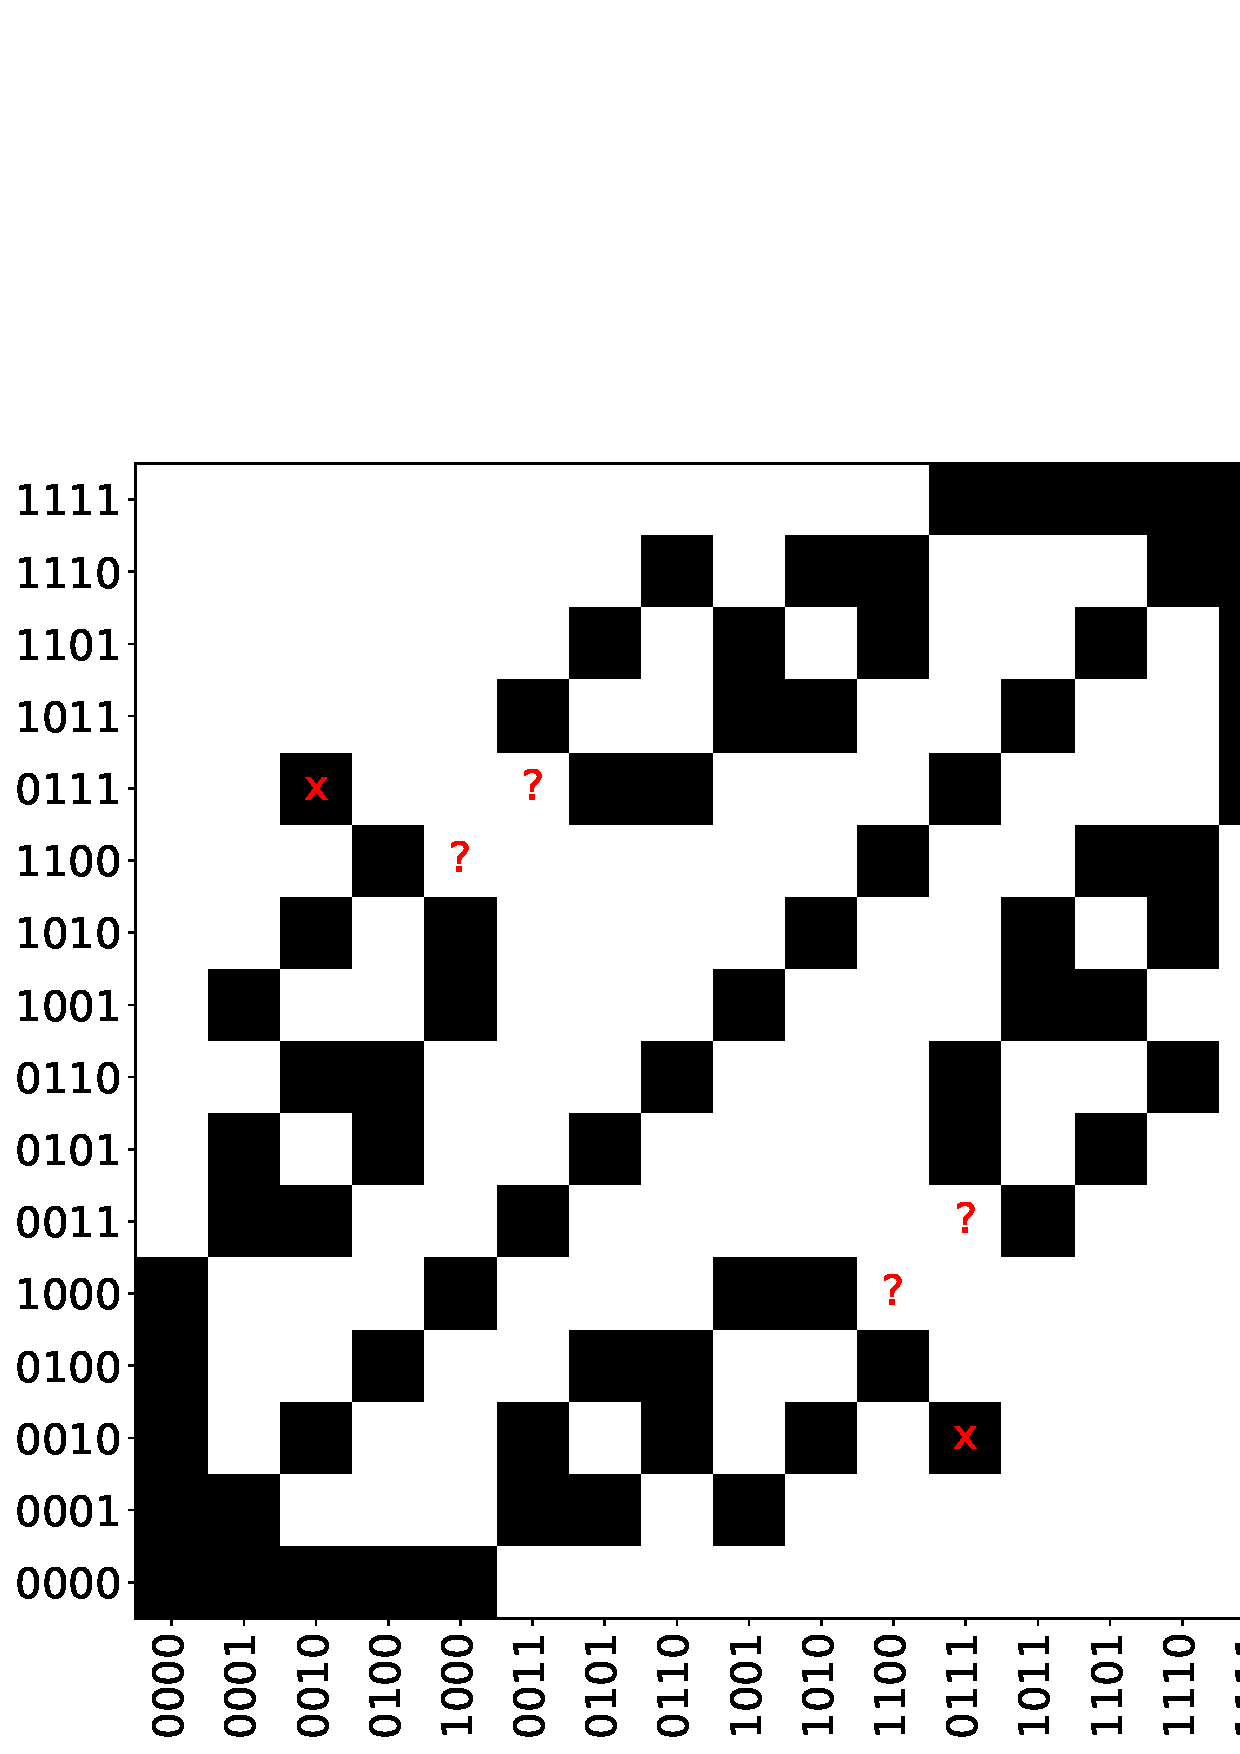
\includegraphics[width=0.95\columnwidth]{distance_matrix.png}
\caption{Hamming distance matrix between two data sets of binary vectors. Values of distance that are less than the median distance value are marked black. Classical simulation of the quantum circuit shows perfect agreement to theoretical calculations and presented on the left figure. Result obtained on the IBM Q Experience ``ibmq\_16\_melbourne'' backend is shown on the right figure. We can see good agreement between the distance matrices calculated classically and on the IBM Q Experience.  [TB: could you put (a) (b) labels as with the other figures. ]} 
\label{fig:distance_matrix}
\end{figure}
%%%%%




We now introduce an optimized algorithm for calculating the matrix of Hamming distances \cite{trugenberger2001} between a sample vector and all cluster vectors, making use of quantum parallelism.  This allows for a simple encoding of the classical information into a quantum register. [TB: allows?]

The overall procedure involves two registers of $n$ qubits each, denoted $\left| X \right\rangle$ and $\left| Y \right\rangle$, along with a single auxiliary qubit $\left| a \right\rangle$. During the whole process, the $\left| Y \right\rangle$ register is used to store the cluster states.  At the beginning and end of the procedure the $\left| X \right\rangle$ register stores the input vectors.  Meanwhile, during the procedure it stores the differences between input vectors and cluster states.

Let us assume we have $k$ input vectors and $l$ cluster states. The $i$th input vector and $j$th cluster vector are respectively denoted as $\left| x_i \right\rangle$, $\left| y_j \right\rangle$. The registers $\left| X \right\rangle$ and $\left| Y \right\rangle$ are initialized to store the input vectors and cluster vectors according to
%
\begin{align}
    \left| X \right\rangle  & = \frac{1}{\sqrt{k}} \sum\limits_{i=1}^{k} \left| x_i \right\rangle,  \\
    \left| Y \right\rangle&  = \frac{1}{\sqrt{l}} \sum\limits_{j=1}^{l} \left| y_j \right\rangle .
    \label{eq:encodnig}
\end{align}
% 
The two registers along with the auxiliary qubit comprise the initial state of the quantum computer according to
%
\begin{equation} 
\left| \psi_0 \right\rangle = 
    \left| X \right\rangle
    \left| Y \right\rangle 
    \left| a \right\rangle
    \label{eq:initial_state}
\end{equation}
%
where $\left| a \right\rangle$ is an auxiliary qubit in the state $\left| 0 \right\rangle$ initially.

Given this initial state we may begin the processing of the problem. We start by applying a CNOT gate between $\left| X \right\rangle$ and $\left| Y \right\rangle$

\begin{align}
    | \psi_1 \rangle & = 
    \mathrm{CNOT} (Y,X)| \psi_0 \rangle \nonumber \\
		& =  
    \frac{1}{\sqrt{kl}} \sum_{i, j=1}^{k} 
    | d^{(1)}_{ij}, \dots, d^{(n)}_{ij} \rangle 
    | y^{(1)}_j, \dots, y^{(n)}_j \rangle
    | 0 \rangle 
\end{align}
%
where $d^\alpha_{ij} = \mathrm{CNOT}(y^\alpha_i, x^\alpha_j)$, $\alpha = 1 \dots n$, and $i,j$ are the qubit indexes in the registers. At this stage of the computation the $\left| X \right\rangle$ no longer stores the input vectors, instead it stores the information about pairwise different qubits between the input vector $\{X\}$ and cluster vector $\{Y\}$. Next, for each pair $\{X\}$ and $\{Y\}$, the accumulated information of all the differences is projected onto the amplitude of the superposed state. This is achieved by applying the Hadamard gate on auxiliary qubit, followed by a controlled phase gate on $\left| Xa \right\rangle$ defined as
%
\begin{equation}
    \label{eq:control_phase_rotation}
    R(\phi) = 
    \begin{pmatrix}
        1 & 0 & 0 & 0 \\
        0 & 1 & 0 & 0 \\
        0 & 0 & 1 & 0 \\
        0 & 0 & 0 & e^{-i\phi}
    \end{pmatrix} .
    \quad \phi = \frac{\pi}{n}
\end{equation}
%
Finally, another Hadamard gate is applied. [TB: on which qubit? I think its better just to describe this using a circuit, rather than describe the steps in words. ]

After the first Hadamard on the ancilla qubit the state is
%
\begin{equation}
    \left| \psi_2 \right\rangle = H_a\left| \psi_1 \right\rangle = 
    \sum\limits_{i, j=1}^{k} 
    \left| d^{(1)}_{ij}, \dots, d^{(n)}_{ij} \right\rangle 
    \left| y^{(1)}_j, \dots, y^{(n)}_j \right\rangle
    \dfrac{(\left| 0 \right\rangle + \left| 1 \right\rangle)}{\sqrt{2}}  .
\end{equation}
%
Applying the controlled phase gate the state then becomes [TB: please define all variables like $ R_{(X,a)} $]
%
\begin{multline}
    \left| \psi_3 \right\rangle = R_{(X,a)}\left(\dfrac{\pi}{n}\right)\left| \psi_2 \right\rangle
    \\ = \dfrac{1}{\sqrt{2}}
				\sum\limits_{i, j=1}^{k} 
				\left| d^{(1)}_{ij}, \dots, d^{(n)}_{ij} \right\rangle 
        \left| y^{(1)}_j, \dots, y^{(n)}_j \right\rangle 
        \left| 0 \right\rangle
        \\ + \dfrac{1}{\sqrt{2}}
				\sum\limits_{i, j=1}^{k}
        \exp\left(\dfrac{-i \pi}{n}\sum\limits_{l=1}^n d^{(l)}_{ij} \right)
        \left| d^{(1)}_{ij}, \dots, d^{(n)}_{ij} \right\rangle 
\\ \times        \left| y^{(1)}_j, \dots, y^{(n)}_j \right\rangle 
        \left| 1 \right\rangle
\end{multline}
%
%
%\\ = \dfrac{1}{\sqrt{2}}
%    \sum\limits_{i, j}^{k}
%    \left| d^{(1)}_{ij}, \dots, d^{(n)}_{ij} \right\rangle 
%        \left| y^{(1)}_j, \dots, y^{(n)}_j \right\rangle 
%        \left| 0 \right\rangle
%        \\ + \dfrac{1}{\sqrt{2}}
%				\sum\limits_{i, j}^{k}
%        \left| R(d^{(1)}_{ij}, 1)\left(\dfrac{\pi}{n}\right), \dots, R(d^{(n)}_{ij}, 1)\left(\dfrac{\pi}{n}\right) \right\rangle 
%        \left| y^{(1)}_j, \dots, y^{(n)}_j \right\rangle 
%        \left| 1 \right\rangle 
%
Applying another Hadamard on the ancilla qubit we obtain
%
\begin{multline}
    \left| \psi_4 \right\rangle = 
    \sum\limits_{i, j=1}^{k} 
    \exp \left(\dfrac{-i \pi}{2n}\sum\limits_{l=1}^n d^{(l)}_{ij} \right)
		\\ \times
        \left[ \cos\left(\dfrac{\pi}{2n}\sum\limits_{l=1}^n d^{(l)}_{ij} \right)
        \left| d^{(1)}_{ij}, \dots, d^{(n)}_{ij} \right\rangle 
        \left| y^{(1)}_j, \dots, y^{(n)}_j \right\rangle 
        \left| 0 \right\rangle\right.
        \\+ 
        \left. i \sin\left(\dfrac{\pi}{2n}\sum\limits_{l=1}^n d^{(l)}_{ij} \right)
        \left| d^{(1)}_{ij}, \dots, d^{(n)}_{ij} \right\rangle 
        \left| y^{(1)}_j, \dots, y^{(n)}_j \right\rangle 
        \left| 1 \right\rangle\right] .
\end{multline}
%
This completes the step for projecting differences between pairs of $\{X\}$ and $\{Y\}$ onto the amplitude of the auxiliary qubit. The process is done in the $x$-basis, achieved by the surrounding Hadamard gates. There are two possible measurement outcomes of the auxiliary qubit.  Each pair of $\{X\}$ and $\{Y\}$ forms a subspace of the Hilbert space, the controlled phase gate ensures to change amplitudes of those outcomes within this subspace depending on how different the spin configurations between $\{X\}$ and $\{Y\}$ are.

At this stage, the information regarding the differences between pairs of $\{X\}$ and $\{Y\}$ is no longer relevant, thus we return to our initial basis for register $\left| X \right\rangle$ by applying pairwise CNOT gates:
%
\begin{multline}
    \left| \psi_f \right\rangle = 
    \mathrm{CNOT} (Y,X)\left| \psi_4 \right\rangle \\=  
    \sum\limits_{i, j=1}^{k} 
    \exp \left(\dfrac{-i \pi}{2n}\sum\limits_{l=1}^n d^{(l)}_{ij} \right)
				\left[ \cos\left(\dfrac{\pi}{2n}\sum\limits_{l=1}^n d^{(l)}_{ij} \right)
        \left| X_i \right\rangle 
        \left| Y_j \right\rangle 
        \left| 0 \right\rangle\right.
        \\+
        \left. i \sin\left(\dfrac{\pi}{2n}\sum\limits_{l=1}^n d^{(l)}_{ij} \right)
        \left| X_i \right\rangle 
        \left| Y_j \right\rangle 
        \left| 1 \right\rangle\right] .
\end{multline}
%
This makes $\{X\}$ store the input vectors again, as in the initial step. It however preserves the amplitudes of the auxiliary qubit which are proportional to how different each pairs of $\{X\}$ and $\{Y\}$ are.

We thus have the Hamming distances encoded into the amplitudes of the final state. From the statistics of the measurement outcomes, the distance matrix between two data sets of binary vectors can be obtained (Fig.~\ref{fig:distance_matrix}). In this case, the biggest amplitude of the measurement result coincides with the smallest Hamming distance when the measurement result of the ancilla qubit is 0. 
If the ancilla qubit is 1, there is an inverse relationship with the measurement result.  [TB: what kind of inverse relationship?]

Measuring the Hamming distance of a particular pair of input vectors $\left| X_i \right\rangle$ and cluster vector $\left| Y_j \right\rangle$ consists of extracting the relevant amplitude from the subspace that those states form, this can be done using the following projection operator
%
\begin{align}
\Pi_{i,j} = &\left| X_i \rangle\langle X_i \right| \otimes \left| X_i \rangle\langle Y_j \right| \otimes I .
\end{align} 
%
Using the above projection operator, the subspace of the Hilbert space formed by a particular pair of input and cluster vectors can be traced out as
%
\begin{align}
    \rho_{i,j} &= \text{Tr}_{1,\dots,2n} (\Pi_{i,j} \left| \psi_f \rangle\langle \psi_f \right| \Pi_{i,j}) .
\end{align}
%
From the state the following two amplitudes for the measurement results can be extracted
%
\begin{align}
    a_0(x_i,y_j) & = \frac{\left\langle 0 |\rho_{i,j}| 0 \right\rangle}{\text{Tr}(\rho_{i,j})}  \\
    a_1(x_i,y_j) & = \frac{\left\langle 1 |\rho_{i,j}| 1 \right\rangle}{\text{Tr}(\rho_{i,j})} .
\end{align}
%
In order to reduce noise we average the measurement results over different states of the ancilla qubit, thus the measured Hamming distance between the input vector $\left| X_i \right\rangle$ and cluster vector $\left| Y_j \right\rangle$ is
%
\begin{align}
    d_{i,j}^H & \propto 1 - \frac{1}{2}(a_0(x_i,y_j) + (1-a_1(x_i,y_j))) .
\end{align}
%
The Hamming distance measured in this way is bounded $0 \leq d_{i,j}^H \leq 1$, where  $0$ indicates that $x_i$ are $y_j$ identical and $1$ means they are completely opposite in terms of their pairwise binary coordinates.

In comparison with the circuits for Hamming distance calculations proposed previously \cite{trugenberger2001}, our method allows one to reduce the number of gates in the circuit and reconstruct all distance matrix in parallel and can be implemented with high fidelity.  We note that at least for the $2n$ one-qubit NOT gates, this depends on the actual realization of the control phase gate in a quantum register at the hardware level.  [TB: don't understand this sentence]

% Please , add comparison of complexities in number of gates for realization between our scheme and previously proposed schemes (one qubit and two qubit separately)  
% ??

 
%\begin{align}
%\\
%\end{align} 
%

%
%\begin{equation}
%\end{equation}
%(a black region indicates if the word occurs in the abstract)

%%%%%
\begin{figure}[t]
\includegraphics[width=0.95\columnwidth]{vectorized_sample.png}
\caption{(a) Representation of the data set of abstracts with the bag-of-words model is shown. Each abstract is represented by a binary vector with 9 elements, corresponding to the 9 words on the horizontal axis. The samples are sorted into groups (QML, MED, BIO) with 3 papers for each tag, for a total of 9 paper.    (b) The Hamming distance between each vectorized abstract is shown as a number in the matrix. 
} 
\label{fig:vectorized_sample}
\end{figure}
%%%%%



















\section{Expeirmental demonstration of QASOFM}

We now show experimental results for a proof-of-concept demonstration of the algorithm introduced in the previous section, on a 16-qubit quantum computer provided by IBM Q Experience.  
We perform unsupervised data clustering for three sets of paper abstracts from three different fields: quantum physics \cite{qml0, qml1, qml2}, medicine \cite{med0, med1, med2} and biology \cite{bio0, bio1, bio2}. Each set consists of three random papers that focus on one of following topics: ``Quantum Machine Learning'' (QML), ``Cancer'' (MED) and ``Gene Expression'' (BIO). Abstracts were vectorized by the bag-of-words model in order to choose most defining words in each data set (see Fig.~\ref{fig:vectorized_sample}). [TB: bag of words reference?]  This model represents text as a multiset ``bag'' of its words taking into account only multiplicity of words. Preparing the bag-of-words we excluded the words that appear only in one abstract and more than in 4 abstracts and we also excluded the word ``level'' from consideration due to the frequent overlap between the clusters because it gives instabilities for both classical and quantum algorithms. We restricted our bag-of-word size to 9 of the most frequent words from the full bags-of-word  due to limitations of the number of qubits. After vectorizing and pre-processing  the data, the clusters are well separated with the Hamming distance.  We observe that distances between the abstracts inside clusters are smaller than distances between the abstracts from different clusters, showing successful self-organization (Fig.~\ref{fig:vectorized_sample}). 


In classical SOFM \cite{kohonen1990}, first a distance calculation between a a sample vector and all cluster vectors is made, then the closest cluster vector is shifted towards the sample vector. The complexity of algorithm, in the sense of the number of distance calculations, scales as $O(LMN)$, where $N$ is number of samples, $M$ is number of randomly sampled cluster vectors, and $L$ is number of the shifts of cluster vectors.  In the QASOFM described in the previous section, distance calculations are realized on a quantum device (i.e. the IBM Q Experience) with the use of circuit presented in Fig. \ref{circuit}. This approach allows one to reduce the number of operations in a number of cluster states with an optimized number of gates that are possible to realize on  quantum computing devices that are currently available. The circuit realized in such a manner that calculation of Hamming distance between the sample vector and all cluster vectors is realized in one operation. The complexity of the quantum assisted SOFM then scales as $O(LN)$. 

In order to check that our algorithm gives the expected results we compare it to classical calculations of the distance matrix on two data sets of binary vectors, as shown in Fig. \ref{fig:distance_matrix}.  We see good agreement between the distance matrices calculated classically and on the IBM Q Experience. The theoretical calculations and classical simulations show perfect agreement with each other. [TB: could you explain why the figures in Fig. 3 are not identical]

An example of the QASOFM learning process is shown in Fig.~\ref{convergence}. Initially, the cluster vectors were randomly chosen (see Fig.~\ref{convergence}) and the label of sample distribution is shown for the zeroth epoch in Fig.~\ref{convergence}(a). In order to prepare a superposition of cluster vectors needed for the calculation of the distance matrix we use the standard initialization of QISKIT library. Each epoch [TB: can you define an epoch exactly?] of the algorithm requires 9 distance calculations in the  quantum implementation (number of samples in general case [TB: use the variable names defined above?]) or 27 distance calculations for classical realization (product of number of samples and number of cluster vectors in general case [TB: use the variable names defined above?]). After the distance calculation from each sample to all cluster vectors at each epoch we label each sample with the index of the closest cluster vector and shift the closest cluster vectors to the sample one. The shift is made by the change of the first binary element in the cluster vectors different from the sample one. The evolution of the labels presented on Fig. ~\ref{convergence}(c).  Good convergence is already observed in the fourth epoch.



[TB: Somehow this feels like the paper ends suddenly without making broader statements.  Do you have any ideas on how to add to this, and develop it a bit more? Just some theory is ok but now it feels like a good start but does not develop the ideas much]

%%%%%
\begin{figure}[t]
\includegraphics[width=0.95\columnwidth]{convergence.png}
\caption{
    (a) Initial random binary vectors of cluster vectors (labeled as C0, C1, C2), for the selected 9 words from the bag of words model. (b) The result of applying our QASOFM implemented on the IBM Q Experience ``ibmq\_16\_melbourne'' backend. Vectors mean cluster elements for BIO, MED, QML groups, for the C0, C1, C2 cluster vectors, respectively. (c) The evolution of label distribution on each learning epoch.
} 
\label{convergence}
\end{figure}
%%%%%



\section{Discussions}
We have developed a quantum assisted SOFM and showed a proof-of-concept experimental demonstration that it can be used to solve clustering problems in an unsupervised manner.  The procedure of solving such clustering problem requires calculating the distance many times in iterative way, which is calculated using a hybrid quantum-classical procedure.  We introduced an optimized circuit for Hamming distance calculations that can be implemented on currently available quantum computing devices with high fidelity. Our quantum circuit performs the distance-computing component of a classical SOFMs algorithm and in this way improve its performance. [TB: Lets include a sentence about the classical and quantum scaling of the problem] 
Due to wide use of classical SOFMs in different areas of modern research and technology, this can give opportunities for the use of QASOFM in practical applications in near term, outperforming classical algorithms.  



\section*{Acknowledgments}
The work is supported by the RFBR-NSFC collaborative program (Grant No. 18-57-53007) and the State assignment (N. 0089-2019-0002). I.D.L. acknowledges support from the Russian Foundation for Basic Research, grant No.19-32-80004 and support from the Foundation for the Advancement of Theoretical Physics and Mathematics “BASIS” No.19-1-5-130-1. T.B. is supported by the Shanghai Research Challenge Fund; New York University Global Seed Grants for Collaborative Research; National Natural Science Foundation of China (61571301, D1210036A); the NSFC Research Fund for International Young Scientists (11650110425, 11850410426); NYU-ECNU Institute of Physics at NYU Shanghai; the Science and Technology Commission of Shanghai Municipality (17ZR1443600); the China Science and Technology Exchange Center (NGA-16-001); and the NSFC-RFBR Collaborative grant (81811530112).





%\section*{Author Contributions}

%I.D.L. and A.N.P. performed the calculations. All authors discussed the results and wrote the paper. 





\section*{Conflict of interest}

The authors declare no conflict of interest.


\section*{Keywords}
quantum self-organizing feature map; quantum machine learning; neural network; quantum unsupervised data clustering; Hamming distance.

\bibliographystyle{naturemag}
\bibliography{bibliography}

%\begin{thebibliography}{99}
%\end{thebibliography}
\end{document}
